\section{Evaluation}
\label{sec:exp}
\begin{figure}[t]
\centering
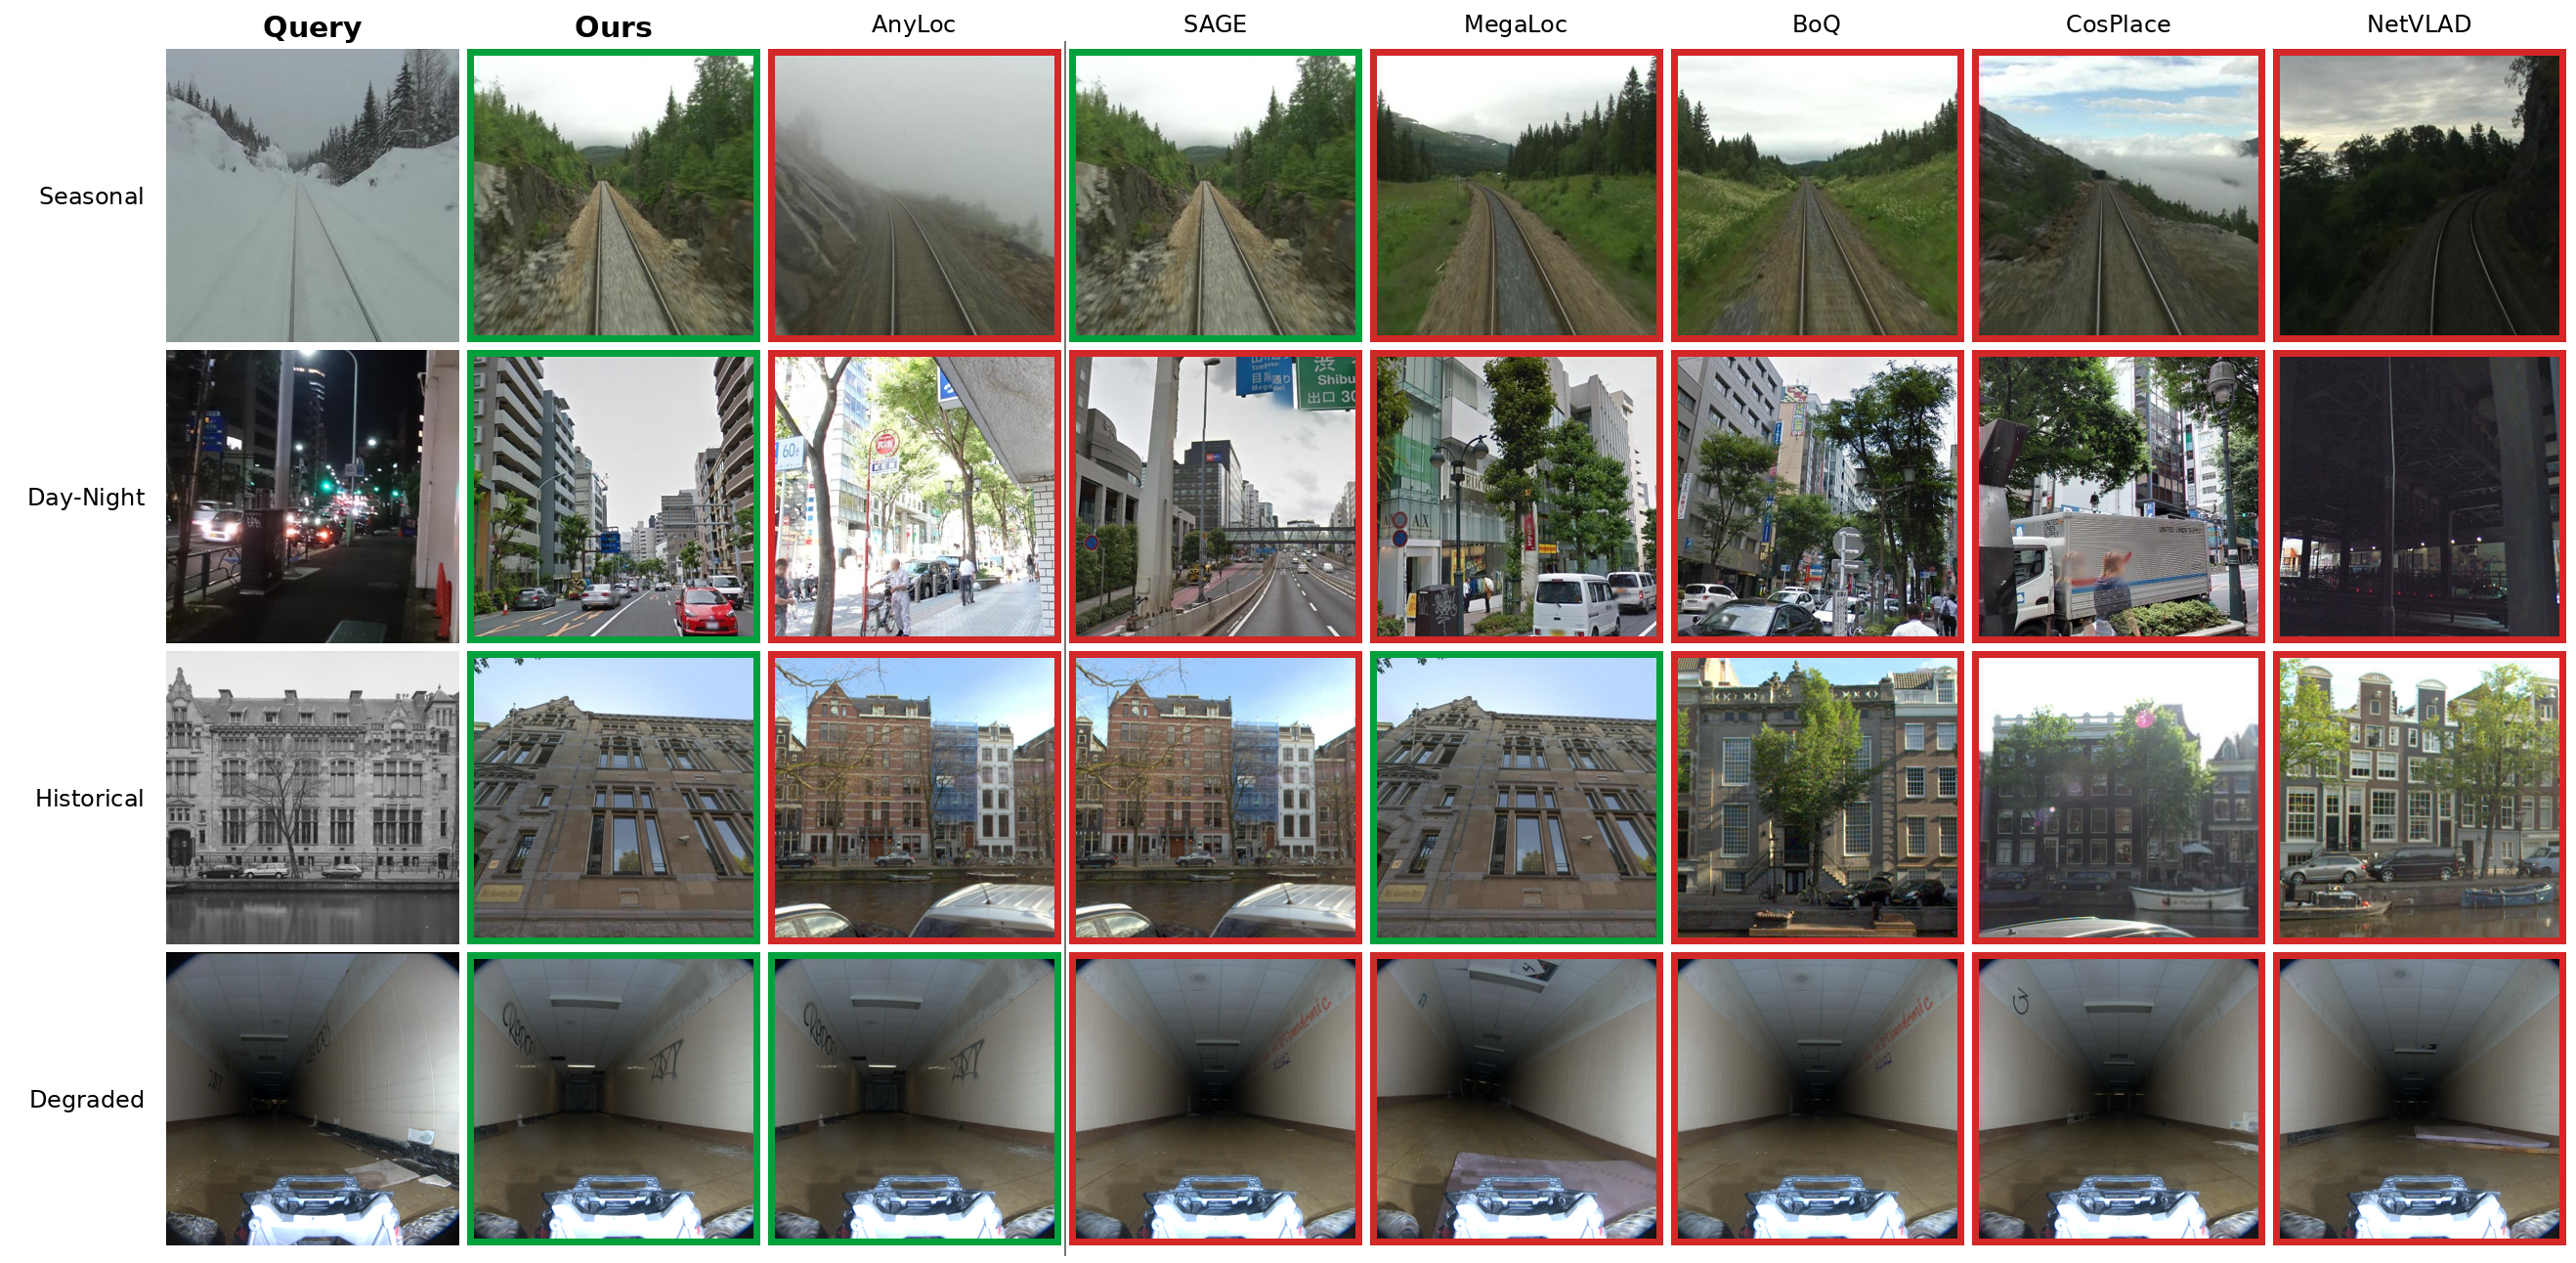
\includegraphics[width=0.82\textwidth]{figures/fig_qualitative.png}
\caption{\textbf{Rank-1 retrievals across benchmark families.} Each method at its own single stage; a green border marks a correct rank-1, red an incorrect one. Training-free methods above the line, the three strongest trained baselines below. Queries are drawn automatically from those our pipeline retrieves correctly, on five axes the one whose correct image sits furthest down every trained baseline's ranking, on the viewpoint axis one the strongest trained baseline still gets right, and on the degraded axis one AnyLoc gets right.}
\label{fig:qual}
\end{figure}

\subsection{Setup and protocol}
\label{sec:setup}
\paragraph{Datasets.} We report thirteen benchmarks spanning eight settings, from urban streets and a seasonal railway to historical photographs and degraded, subterranean, indoor, aerial and underwater imagery. Table~\ref{tab:datasets} says what each benchmark asks of a place representation; Appendix~\ref{app:protocol} gives the split, the database and query counts, the ground-truth distance and the three conventions on which the published literature disagrees.

\begin{table}[t]
\caption{\textbf{The thirteen benchmarks.} What each one asks of a place representation. Splits, database and query counts and ground-truth distances are in Appendix~\ref{app:protocol}.}
\label{tab:datasets}
\centering
{\footnotesize\setlength{\tabcolsep}{4pt}%
\begin{tabular}{ll}
\toprule
Benchmark & What it tests \\
\midrule
\multicolumn{2}{l}{\emph{Urban, street level}} \\
Pitts30k, Pitts250k & viewpoint change in a dense city survey \\
Tokyo 24/7 & the same places by day, at dusk and at night \\
MSLS-val & a moving camera across cities, seasons and weather \\
St Lucia & a vehicle repeating a suburban route \\
Oxford RobotCar & a vehicle repeating a route months apart \\
Nordland & one railway line in four seasons, no viewpoint change \\
AmsterTime & historical photographs against present-day ones \\
\midrule
\multicolumn{2}{l}{\emph{Beyond street level}} \\
Hawkins, Laurel Caverns & subterranean corridors, little texture, poor light \\
17 Places, Baidu Mall & indoor scenes that repeat themselves \\
Gardens Point & an indoor route walked by day and by night \\
VP-Air, Nardo-Air, Nardo-Air R & aerial imagery, the last one rotated \\
Mid-Atlantic Ridge & deep-sea imagery from a hydrothermal vent \\
\bottomrule
\end{tabular}%
}
\end{table}



\paragraph{Implementation details.} One configuration is used for every benchmark. Tokens are the value facet of a frozen DINOv3 ViT-L/16 at block $20$ or ViT-7B/16 at block $32$, taken at $768$px for $2{,}304$ patches and reduced to $C{=}512$ channels by a token-PCA. Weights are $w_i{=}1/n_i$ at $\tau{=}0.5$, computed on the full token set. Stage 1 stores $F^{\top}WF$ built from each image's $1024$ highest-weight tokens, $\ell_2$-normalized and reduced to $2048$ dimensions by a whitened descriptor-PCA, and scans to a shortlist of $K{=}\min(1000,|\mathcal{D}|)$ over the deployment database $\mathcal{D}$. Stage 2 re-ranks by \eqref{eq:stage2} at $\theta{=}0.65$, scoring those $1024$ tokens on the urban benchmarks and all $2{,}304$ on the environment sets (Appendix~\ref{app:s2grid}). The DINOv2 rows run at each backbone's native resolution. Nothing is fitted outside $\mathcal{D}$: the token-PCA and the descriptor whitening are estimated from a few hundred of its unlabelled images, neither using a label. All runs are on one H100, and layer, facet, shortlist depth and every constant are swept in Appendix~\ref{app:hyper}.

\paragraph{Evaluation metric.} A return counts as correct when it lies within the benchmark's distance of the query's true location, and we report Recall@$1$, the share of queries whose top return is correct.

\subsection{Comparison with state-of-the-art}
\label{sec:sota}
We compare our two-stage pipeline with previous state of the art, both trained and training-free, at each method's own published setting.

\begin{table}[t]
\caption{\textbf{Training-free methods against ours on all seventeen benchmarks.} Recall@1, one deployed configuration throughout; the urban block re-ranks $1024$ tokens per image, the environment block all $2{,}304$. \emph{Dim} is the first-stage descriptor dimensionality, as evaluated. \textsc{CLS token} is the frozen DINOv2-L class token retrieved by cosine. Baseline cells are published numbers, or our run of the released code where the paper omits the benchmark; ``---'' marks a run not yet complete. $^{d}$AnyLoc's VP-Air figure may omit the $10{,}000$ distractors ours carries. $^{\dagger}$two-stage. Bold $=$ best, \underline{underline} $=$ second, within each block.}
\label{tab:breadth}
\centering
{\scriptsize\setlength{\tabcolsep}{2.0pt}\renewcommand{\arraystretch}{0.92}%
\begin{tabular}{ll ccccccccc|c}
\toprule
\multicolumn{12}{l}{\emph{Standard benchmarks (urban)}} \\
Method & Dim & Pitts250k & Pitts30k & Tokyo24/7 & MSLS-val & Nordland & St Lucia & Oxford & AmsterTime & & mean \\
\midrule
CLS token & 1024 & 80.3 & 78.7 & 46.0 & 37.8 & 15.9 & 81.5 & 25.6 & 45.8 &  & 51.5 \\
GeM & 1024 & 80.4 & 78.5 & 69.8 & 36.0 & 15.0 & 74.2 & 71.7 & 27.9 &  & 56.7 \\
AnyLoc & 49152 & 81.5 & 87.7 & 90.5 & 49.2 & 20.2 & 96.2 & \textbf{99.5} & 44.6 &  & 71.2 \\
EffoVPR-ZS$^{\dagger}$ & 1024 & 93.4 & 89.4 & 90.8 & 70.3 & 57.9 & 97.8 & 77.0 & 65.8 &  & 80.3 \\
SegVLAD-PreT & 49152 & --- & 86.7 & --- & --- & --- & --- & 73.8 & 62.4 &  & --- \\
\midrule
Ours\,\emph{v2}$^{\dagger}$ & 2048 & \underline{95.7} & \underline{92.5} & \underline{97.5} & \underline{89.0} & \underline{83.0} & \underline{99.1} & \underline{99.0} & \underline{68.1} &  & \underline{90.5} \\
Ours\,\emph{v3}$^{\dagger}$ & 2048 & \textbf{96.1} & \textbf{93.7} & \textbf{98.4} & \textbf{89.3} & \textbf{96.6} & \textbf{99.7} & \underline{99.0} & \textbf{73.6} &  & \textbf{93.3} \\
\midrule\midrule
\multicolumn{12}{l}{\emph{Nine environments}} \\
Method & Dim & Hawk & Laurel & 17Pl & Gard & Baidu & N-Air & N-AirR & VP-Air & M-Atl & mean \\
\midrule
CLS token & 1024 & 26.3 & 50.9 & 61.1 & 75.0 & 43.1 & 56.3 & 76.1 & 38.0 & 24.8 & 50.2 \\
GeM & 1024 & 56.8 & 50.9 & 64.0 & 89.5 & 46.2 & 81.7 & 85.9 & 42.2 & 23.8 & 60.1 \\
AnyLoc & 49152 & \underline{65.2} & 61.6 & 65.0 & 95.5 & 75.2 & 76.1 & 85.9 & 66.7$^{d}$ & 34.6 & 69.5 \\
EffoVPR-ZS$^{\dagger}$ & 1024 & 38.1 & 67.0 & \textbf{65.5} & \underline{97.5} & 75.9 & \underline{83.1} & 88.7 & 65.7 & \underline{36.6} & 68.7 \\
SegVLAD-PreT & 49152 & 56.8 & 26.8 & 64.8 & 91.5 & 78.5 & 45.1 & 40.9 & 69.8 & 22.8 & 55.2 \\
\midrule
Ours\,\emph{v2} & 2048 & \textbf{67.0} & \textbf{83.0} & \textbf{65.5} & \textbf{99.5} & \textbf{84.5} & \underline{83.1} & \underline{94.4} & \underline{72.1} & \textbf{37.6} & \underline{76.3} \\
Ours\,\emph{v3} & 2048 & 61.0 & \underline{75.9} & \underline{65.3} & \textbf{99.5} & \underline{83.5} & \textbf{91.5} & \textbf{97.2} & \textbf{77.6} & \textbf{37.6} & \textbf{76.6} \\
\bottomrule
\end{tabular}%
}
\end{table}

Table~\ref{tab:breadth} sets ours against every training-free method on all seventeen benchmarks. On the urban block we lead the best prior training-free number on all eight, by $+4.3$ R@1 on Pitts30k and $+7.6$ on Tokyo 24/7 where the comparison is closest, and by $+38.7$ on Nordland, whose seasonal change is the hardest condition in the block; the two rows differ by $2.8$ mean R@$1$, almost all of it on Nordland, where the frozen features carry the seasonal change on their own. On the nine environments we take the best number on eight and the second on the ninth, for a mean of $76.6$ against $69.5$ for AnyLoc, the strongest training-free alternative, whose descriptor is $24\times$ larger.

\label{sec:ood}

\begin{table}[t]
\caption{\textbf{Trained methods against ours on the nine environments, two stages against two stages.} R@1 under the same deployed configuration, re-ranking all $2{,}304$ tokens; the training-free comparison is in Table~\ref{tab:breadth}. \emph{Dim} is the first-stage descriptor dimensionality, as evaluated. Each method as published: $^{\dagger}$after its own re-ranker, $^{\ddag}$without the cross-image encoder. Bold $=$ best, \underline{underline} $=$ second.}
\label{tab:ood}
\centering
{\scriptsize\setlength{\tabcolsep}{2pt}%
\begin{tabular}{llccccccccc|c}
\toprule
 & & Degr.\ & SubT & \multicolumn{3}{c}{Indoor} & \multicolumn{3}{c}{Aerial} & UW & \\
\cmidrule(lr){3-11}
Method & Dim & Hawk & Laurel & 17Pl & Gard & Baidu & N-Air & N-AirR & VP-Air & M-Atl & mean \\
\midrule
\multicolumn{12}{l}{\emph{Trained / fine-tuned}} \\NetVLAD & 32768 & 38.1 & 42.9 & 63.8 & 66.0 & 57.8 & 9.9 & 39.4 & 14.7 & 26.7 & 39.9 \\
SFRS & 4096 & 29.7 & 21.4 & 59.1 & 55.0 & 51.3 & 0.0 & 47.9 & 9.4 & 9.9 & 31.5 \\
CosPlace & 2048 & 33.9 & 25.9 & 63.3 & 84.5 & 47.1 & 0.0 & 76.1 & 10.4 & 32.7 & 41.5 \\
MixVPR & 4096 & 26.3 & 32.1 & 63.8 & 92.0 & 68.4 & 39.4 & 78.9 & 12.9 & 24.8 & 48.7 \\
EigenPlaces & 2048 & 28.8 & 27.7 & 63.8 & 86.0 & 66.6 & 12.7 & \textbf{100.0} & 13.1 & 29.7 & 47.6 \\
R2Former$^{\dagger}$ & 256 & 17.8 & 30.4 & 63.8 & 84.0 & 74.7 & 26.8 & 83.1 & 15.0 & 22.8 & 46.5 \\
SALAD & 8448 & 38.1 & 46.4 & 64.3 & 96.5 & 69.9 & 53.5 & 94.4 & 24.0 & 15.8 & 55.9 \\
CricaVPR$^\ddag$ & 10752 & 28.0 & 34.8 & 64.0 & 94.0 & 65.8 & 45.1 & \textbf{100.0} & 19.9 & 27.7 & 53.3 \\
SelaVPR$^{\dagger}$ & 1024 & 25.4 & 53.6 & 63.3 & 94.5 & 68.5 & 59.1 & 83.1 & 32.6 & 21.8 & 55.8 \\
BoQ & 12288 & 33.9 & 60.7 & 64.3 & \underline{98.0} & 77.4 & 62.0 & 91.5 & 29.5 & 35.6 & 61.4 \\
CliqueMining & 8448 & 22.9 & 38.4 & \underline{65.3} & 93.0 & 69.1 & 62.0 & 84.5 & 22.9 & 35.6 & 54.9 \\
SuperVLAD$^\ddag$ & 3072 & 37.3 & 51.8 & 64.8 & 95.5 & 70.3 & 14.1 & 88.7 & 23.8 & 13.9 & 51.1 \\
VLAD-BuFF & 4096 & 37.3 & 33.9 & 64.5 & 96.5 & 76.4 & 57.7 & 88.7 & 33.3 & 27.7 & 57.4 \\
SelaVPR++$^{\dagger}$ & 2048 & 21.2 & 35.7 & 65.0 & 95.5 & 73.6 & 81.7 & 87.3 & 42.7 & 27.7 & 58.9 \\
MegaLoc & 8448 & 37.3 & 55.4 & 64.8 & 95.5 & 79.4 & \underline{85.9} & 81.7 & 45.6 & \textbf{40.6} & 65.1 \\
FoL$^{\dagger}$ & 8448 & 36.4 & 54.5 & \underline{65.3} & 97.0 & 78.9 & 77.5 & \underline{98.6} & 46.7 & 25.7 & 64.5 \\
SAGE$^\ddag$ & 8448 & 27.1 & 46.4 & 64.0 & 93.5 & 74.6 & \underline{85.9} & 84.5 & 39.1 & 24.8 & 60.0 \\
\midrule
\multicolumn{12}{l}{Ours \emph{--- training-free, coarse retrieval with \textsc{MaxSim} interaction}} \\
Ours\,\emph{v2} & 2048 & \textbf{67.0} & \textbf{83.0} & \textbf{65.5} & \textbf{99.5} & \textbf{84.5} & 83.1 & 94.4 & \underline{72.1} & \underline{37.6} & \underline{76.3} \\
Ours\,\emph{v3} & 2048 & \underline{61.0} & \underline{75.9} & \underline{65.3} & \textbf{99.5} & \underline{83.5} & \textbf{91.5} & 97.2 & \textbf{77.6} & \underline{37.6} & \textbf{76.6} \\
\bottomrule
\end{tabular}%
}
\end{table}

Table~\ref{tab:ood} takes the same configuration off street view, to degraded, subterranean, indoor, aerial and underwater imagery, with every method given a second stage of its own so that two-stage is compared against two-stage. We take the best number on eight of the nine environments and the second on the ninth, for a mean of $76.6$ against $65.1$ for the strongest trained method (MegaLoc). The margins are largest where a single descriptor has least to work with: $67.0$ against $38.1$ on the degraded Hawkins corridor, $83.0$ against $60.7$ in Laurel Caverns, and $77.6$ against $46.7$ on VP-Air, the aerial set with the deepest database. The two backbones differ by $0.3$ R@1 on the mean, so the result rests on the pipeline rather than on backbone scale.

Figure~\ref{fig:qual} shows one query per benchmark family. Where the trained baselines return a different place under seasonal change, illumination change or a degraded interior, our pipeline returns the correct image at rank one.


\subsection{Ablation study}
\label{sec:swap}
Table~\ref{tab:w-signal} asks what the weight should read. Every row changes only $w$ and leaves the backbone, the shortlist and the scoring rule untouched. Self-similarity, down-weighted, leads at $93.03$ R@1; class-token attention is the closest alternative at $92.62$; reversing the direction of a patch-graph signal costs $9.1$; token norm, inverse document frequency and spatial verification all sit at or below the unweighted baseline of $87.62$.

\begin{table}[t]
\caption{\textbf{Which patch-importance signal.} Pitts30k, $6816$ queries, DINOv2-G layer $31$, weighted \textsc{MaxSim} over an AnyLoc top-$100$ pool. Every row changes only $w$. \emph{Source} names the work the signal is taken from.}
\label{tab:w-signal}
\centering
{\footnotesize
\begin{tabular}{ll c l}
\toprule
Signal for $w$   &   Source   &  R@1 &   \\
\midrule
none (bare \textsc{MaxSim})   &   ---   &  87.62 &   baseline \\
\midrule
\textbf{self-similarity, down-weighted}   &   this work   &  \textbf{93.03} &   best \\
class-token attention, up-weighted    &    \citep{effovpr}    &  92.62 &    close second \\
patch-graph centrality, up-weighted    &    SAP    &  90.44 &    works, weaker \\
\midrule
patch-graph centrality, \emph{down}-weighted   &   ---   &  83.94 &   direction reversed \\
token norm, up-weighted    &    \citep{registers}    &  87.72 &    neutral \\
token norm, down-weighted    &    \citep{registers}    &  87.53 &    neutral \\
inverse document frequency    &    Video Google    &  86.53 &    below baseline \\
cross-referencing    &    DeepEMD    &  81.78 &    below baseline \\
rapid spatial verification    &    \citep{patchnetvlad}    &  84.24 &    below baseline \\
\bottomrule
\end{tabular}%
}\end{table}

Table~\ref{tab:stage2swap} isolates our second stage by dropping it into other pipelines: each method keeps its backbone, resolution and shortlist, and only the scoring rule changes. The upper block re-ranks the shortlist of the four methods that ship a second stage of their own, and all four improve on the nine-environment mean, FoL by $+5.5$, R2Former $+5.6$, SelaVPR $+9.7$ and SelaVPR++ $+12.5$ R@1, better on $28$ of the $36$ cells. The lower block adds it where a method ships none, and all eight improve, by $+9.1$ (MegaLoc) to $+17.8$ (SuperVLAD), better on $63$ of the $72$ cells. The gain is largest exactly where a single descriptor is weakest, and the rule needs no training, no fitted part and no access to a method's internals.

\begin{table}[t]
\caption{\textbf{Our second stage on other methods' first stages.} Each figure is what the method publishes, after its own re-ranker in the upper block and from its global descriptor in the lower; the subscript is the change under \eqref{eq:stage2}, replacing that re-ranker or added where there is none. Backbone, resolution and shortlist stay the method's own.}
\label{tab:stage2swap}
\centering
{\scriptsize\setlength{\tabcolsep}{2pt}%
\resizebox{\textwidth}{!}{%
\begin{tabular}{llccccccccc|c}
\toprule
& & Degr.\ & SubT & \multicolumn{3}{c}{Indoor} & \multicolumn{3}{c}{Aerial} & UW & \\
\cmidrule(lr){3-11}
Method   &   Backbone   &   Hawk   &   Laurel   &  17Pl &   Gard   &   Baidu   &   N-Air   &   N-AirR   &   VP-Air   & M-Atl &   mean \\
\midrule
\multicolumn{12}{l}{\emph{Replacing each method's own re-ranking stage}} \\
FoL            & DINOv2-L   & 36.4\dlt{+14.4} & 54.5\dlt{+18.7} & 65.3\dlt{-0.5} & 97.0\dlt{+1.0} & 78.9\dlt{+2.4} & 77.5\dlt{+4.2} & 98.6\dlt{-4.2} & 46.7\dlt{+10.1} & 25.7\dlt{+3.0} & 64.5\dltg{+5.5} \\
SelaVPR++      & DINOv2-L   & 21.2\dlt{+44.9} & 35.7\dlt{+39.3} & 65.0\dlt{-0.0} & 95.5\dlt{+3.0} & 73.6\dlt{+8.0} & 81.7\dlt{-5.6} & 87.3\dlt{+2.8} & 42.7\dlt{+25.0} & 27.7\dlt{-4.9} & 58.9\dltg{+12.5} \\
SelaVPR        & DINOv2-L   & 25.4\dlt{+38.2} & 53.6\dlt{+13.4} & 63.3\dlt{+2.5} & 94.5\dlt{+1.5} & 68.5\dlt{+7.5} & 59.1\dlt{+1.5} & 83.1\dlt{+1.4} & 32.6\dlt{+23.5} & 21.8\dlt{-2.0} & 55.8\dltg{+9.7} \\
R2Former       & DeiT-S     & 17.8\dlt{+22.9} & 30.4\dlt{+16.1} & 63.8\dlt{+0.7} & 84.0\dlt{-3.5} & 74.7\dlt{+0.6} & 26.8\dlt{+5.6} & 83.1\dlt{-1.4} & 15.0\dlt{+2.8} & 22.8\dlt{+6.9} & 46.5\dltg{+5.6} \\
\midrule
\multicolumn{12}{l}{\emph{Added to methods that provide no re-ranking stage}} \\
SALAD                & DINOv2-B   & 38.1\dlt{+24.6} & 46.4\dlt{+25.9} & 64.3\dlt{+1.0} & 96.5\dlt{+3.0} & 69.9\dlt{+12.1} & 53.5\dlt{+29.6} & 94.4\dlt{+1.4} & 24.0\dlt{+22.1} & 15.8\dlt{+14.9} & 55.9\dltg{+14.9} \\
CricaVPR$^\ddag$     & DINOv2-B   & 28.0\dlt{+31.4} & 34.8\dlt{+32.1} & 64.0\dlt{+1.5} & 94.0\dlt{+4.5} & 65.8\dlt{+18.9} & 45.1\dlt{+18.3} & 100.0\dlt{-8.5} & 19.9\dlt{+22.8} & 27.7\dlt{+8.9} & 53.3\dltg{+14.4} \\
BoQ                  & DINOv2-B   & 33.9\dlt{+33.1} & 60.7\dlt{+16.1} & 64.3\dlt{+0.7} & 98.0\dlt{+1.0} & 77.4\dlt{+6.5} & 62.0\dlt{+31.0} & 91.5\dlt{-8.5} & 29.5\dlt{+24.9} & 35.6\dlt{-5.0} & 61.4\dltg{+11.1} \\
CliqueMining         & DINOv2-B   & 22.9\dlt{+39.8} & 38.4\dlt{+35.7} & 65.3\dlt{-0.2} & 93.0\dlt{+6.0} & 69.1\dlt{+13.8} & 62.0\dlt{+8.5} & 84.5\dlt{+11.3} & 22.9\dlt{+26.2} & 35.6\dlt{-1.0} & 54.9\dltg{+15.6} \\
SuperVLAD$^\ddag$    & DINOv2-B   & 37.3\dlt{+23.7} & 51.8\dlt{+21.4} & 64.8\dlt{+1.5} & 95.5\dlt{+3.5} & 70.3\dlt{+15.1} & 14.1\dlt{+60.6} & 88.7\dlt{-9.9} & 23.8\dlt{+23.4} & 13.9\dlt{+20.8} & 51.1\dltg{+17.8} \\
MegaLoc              & DINOv2-B   & 37.3\dlt{+33.1} & 55.4\dlt{+17.0} & 64.8\dlt{+1.2} & 95.5\dlt{+3.0} & 79.4\dlt{+5.7} & 85.9\dlt{+1.4} & 81.7\dlt{+9.9} & 45.6\dlt{+16.3} & 40.6\dlt{-5.9} & 65.1\dltg{+9.1} \\
SAGE$^\ddag$         & DINOv2-L   & 27.1\dlt{+37.3} & 46.4\dlt{+26.8} & 64.0\dlt{+0.5} & 93.5\dlt{+5.0} & 74.6\dlt{+6.7} & 85.9\dlt{-9.9} & 84.5\dlt{+5.6} & 39.1\dlt{+26.3} & 24.8\dlt{-2.0} & 60.0\dltg{+10.7} \\
VLAD-BuFF            & DINOv2-B   & 37.3\dlt{+23.7} & 33.9\dlt{+33.0} & 64.5\dlt{+1.0} & 96.5\dlt{+3.0} & 76.4\dlt{+8.1} & 57.7\dlt{+9.9} & 88.7\dlt{+5.6} & 33.3\dlt{+20.1} & 27.7\dlt{+7.9} & 57.4\dltg{+12.5} \\
\bottomrule
\end{tabular}%
}%
}
\end{table}
